\section{Auswertung}

In der folgenden Auswertung werden zuerst die beiden Relaxationszeiten $T\ua{1}$
sowie $T\ua{2}$ bestimmt. Mithilfe von $T\ua{2}$ kann dann die Diffusionskonstante $D$ sowie
der Molekülradius bestimmt werden. Der Molekülradius wird am Ende zudem mit
den Radien verglichen, die sich aus dem Molekulargewicht und dem Van-der-Waals-Kovolumen
ergeben.

\subsection{Bestimmung der longitudinalen Relaxationszeit}% \text{$T\ua{1}$}}

Die aufgenommenen Daten für die Bestimmung von $T\ua{1}$ sind Tabelle \ref{tab:T1}
eingetragen sowie in Abbildung \ref{fig:T1} grafisch dargestellt.
\begin{table}
  \centering
  \caption{Messdaten für die Spannungamplituden des ersten Echos bei verschiedenen
  Pulsabständen.}
  \label{tab:T1}
  \begin{tabular}{S  S | S  S}
    \toprule
    {$\tau / \si{ms}$} & {$U / \si{mV}$} & {$\tau /\si{ms}$} & {$U / \si{mV}$} \\
    \midrule
    1  & -785 & 100  & -633 \\
    2  & -780 & 200  & -565   \\
    3  & -765 & 500  & -395   \\
    5  & -745 & 1000 & -195   \\
    8  & -745 & 1500 &   35   \\
    9  & -735 & 2000 &  118   \\
    13 & -730 & 4000 &  612   \\
    20 & -715 & 7000 &  643 \\
    50 & -665 & 9000 &  700   \\
    75 & -648 & &           \\
    \bottomrule
  \end{tabular}
\end{table}

Um $T\ua{1}$ zu bestimmen werden die experimentellen Daten an eine Exponentialfunktion
der folgenden Form gefittet:
\begin{equation}
  U(t) = M\ua{0}(1-2\exp{(-\frac{t}{T_1})})+M\ua{1}.
\end{equation}
Für die verschiedenen Parameter ergeben sich damit folgende Werte:
\begin{align}
  M\ua{0} &= (0.73\pm0.02)\,\si{V} \\
  M\ua{1} &= (0.04\pm0.03)\,\si{V} \\
  T\ua{1} &= (1.54\pm0.12)\,\si{s}.
\end{align}
\begin{figure}
  \centering
  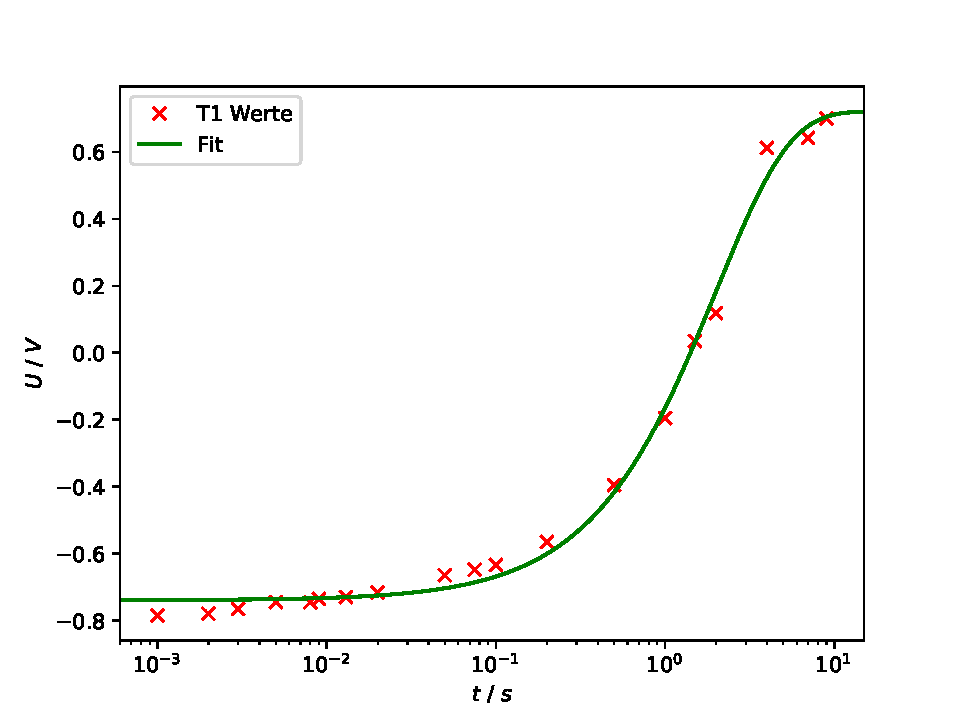
\includegraphics[width=0.8\textwidth]{Plots2/T1.pdf}
  \caption{Gemessene Signalhöhe des Echos gegen den zeitlichen Abstand der beiden Pulse.}
  \label{fig:T1}
\end{figure}

\subsection{Bestimmung der transversalen Relaxationszeit}% \text{$T\ua{2}$}}
\label{subsec:T2}

Um die transversale Relaxationszeit $T\ua{2}$ zu bestimmen wird das Meiboom-Gill Verfahren
verwendet. Zudem ist in Abbildung \ref{fig:T2CP} einmal die Burstsequenz mit dem
Carr-Purcell-Verfahren dargestellt.
\begin{figure}\centering
  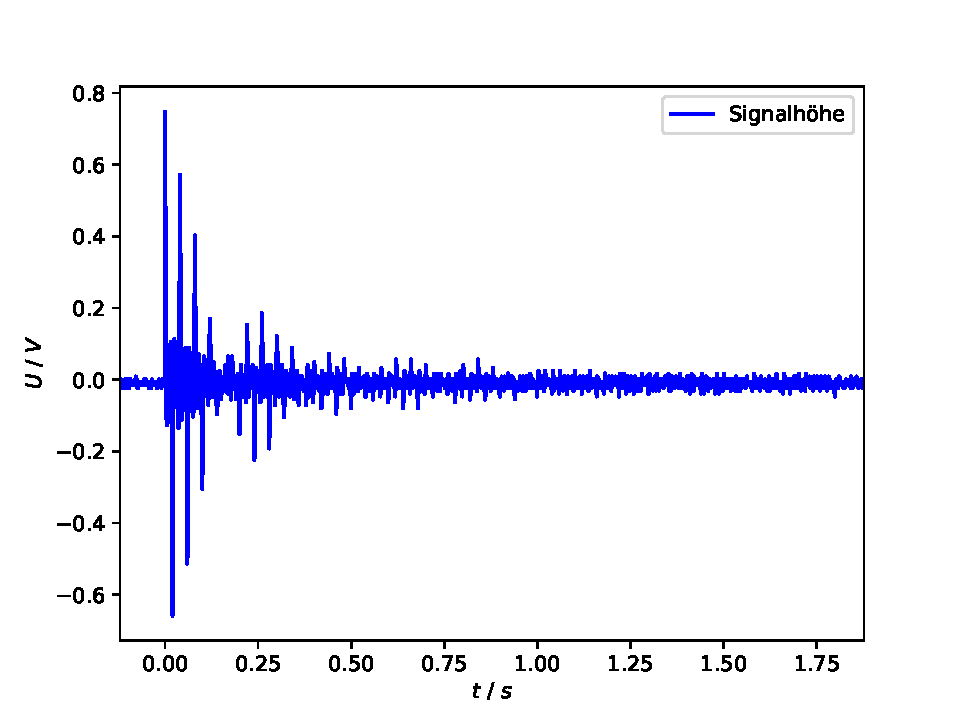
\includegraphics[width=0.8\textwidth]{Plots2/T2CP.pdf}
  \caption{Signale der transversalen Magnetisierung mit der Carr-Purcell-Methode
  bei einem Pulsabstand von $\tau = \SI{2}{ms}$. }
  \label{fig:T2CP}
\end{figure}
In Abbildung \ref{fig:T2} ist die Burstsequenz mit der Meiboom-Gill Methode
dargestellt. Um $T\ua{2}$ zu bestimmen, werden alle Spannungsamplitudem bei
ganzzahligen Vielfachen von $2\tau$ verwendet. Die verwendeten Peaks sind als
rot gefärbte Datenpunkte markiert. Mit den in Tabelle \ref{tab:T2Ex} eingetragenen
extrahierten Daten wird ein Fit der Form
\begin{equation}
  U(t) = M\ua{0}\cdot\exp{(-\frac{t}{T\ua{2}})}+M\ua{1}
\end{equation}
durchgeführt.
Für die verschiedenen Parameter ergeben sich dabei folgende Werte:
\begin{align*}
  M\ua{0} &= (0.59\pm0.02)\,\si{V}\\
  M\ua{1} &= (0.04\pm0.03)\,\si{V}\\
  T\ua{2} &= (1.54\pm0.12)\,\si{s}.
\end{align*}
Die extrahierten Messwerte sowie der FIt sind noch einmal in Abbildung \ref{fig:T2Log} mit
logarithmierter Y-Achse dargestellt.
\begin{figure}
  \centering
  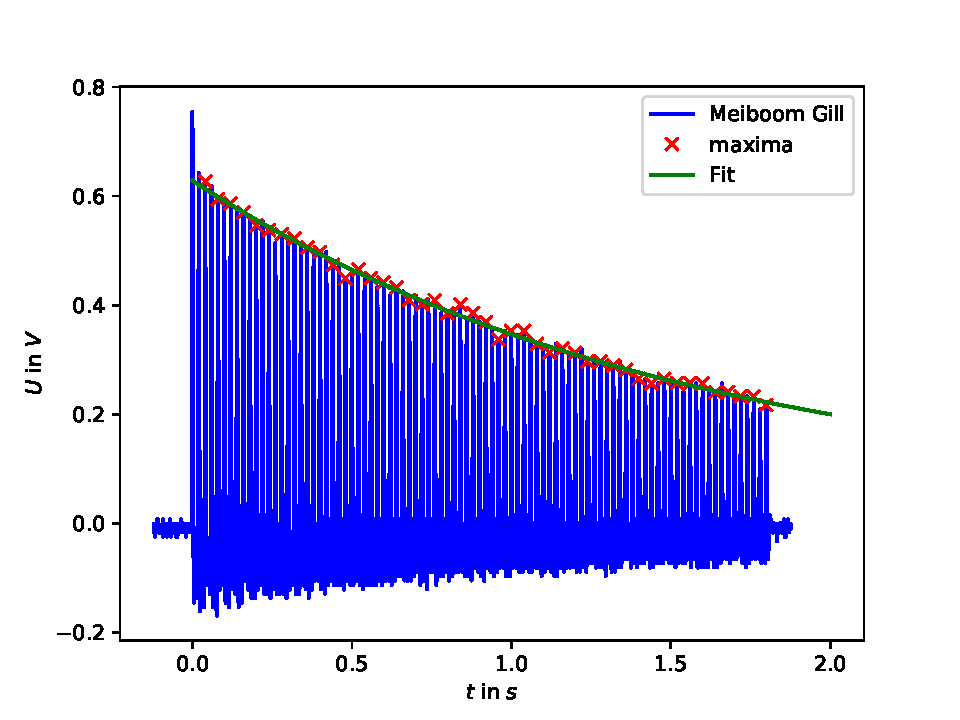
\includegraphics[width=0.8\textwidth]{Plots2/T2.pdf}
  \caption{Die aufgenommenen Spannungsamplituden unter Verwendung der
  Meiboom-Gill-Methode bei einem Pulsabstand von $\tau = \SI{2}{ms}$.}
  \label{fig:T2}
\end{figure}
\begin{figure}
  \centering
  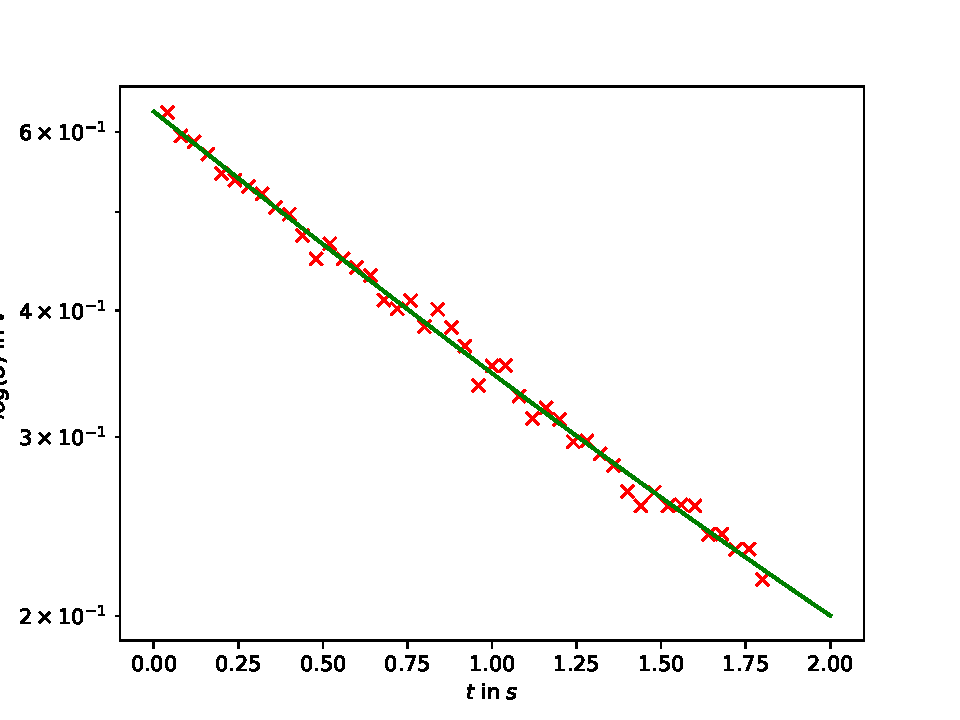
\includegraphics[width=0.8\textwidth]{Plots2/T2Log.pdf}
  \caption{Darstellung der extrahierten Punkte mit logarithmierter Y-Achse.}
  \label{fig:T2Log}
\end{figure}
\begin{table}
  \centering
  \caption{Extrahierte Messdaten für die Spannungamplituden bei Verwendung der Meiboom-Gill-Methode}
  \label{tab:T2Ex}
  \begin{tabular}{S  S | S  S | S S}
    \toprule
    {$\tau / \si{ms}$} & {$U / \si{mV}$} & {$\tau /\si{ms}$} & {$U / \si{mV}$}
    & {$\tau /\si{ms}$} & {$U / \si{mV}$} \\
    \midrule
    0.00 & 0.754 & 0.63 & 0.418 & 1.22 & 0.321 \\
    0.02 & 0.642 & 0.64 & 0.433 & 1.24 & 0.297 \\
    0.04 & 0.627 & 0.66 & 0.425 & 1.26 & 0.297 \\
    0.05 & 0.618 & 0.68 & 0.410 & 1.28 & 0.297 \\
    0.08 & 0.594 & 0.70 & 0.418 & 1.30 & 0.297 \\
    0.10 & 0.586 & 0.72 & 0.401 & 1.32 & 0.289 \\
    0.12 & 0.586 & 0.74 & 0.409 & 1.34 & 0.297 \\
    0.14 & 0.578 & 0.76 & 0.409 & 1.36 & 0.281 \\
    0.16 & 0.570 & 0.78 & 0.385 & 1.38 & 0.273 \\
    0.18 & 0.554 & 0.80 & 0.385 & 1.40 & 0.265 \\
    0.20 & 0.546 & 0.82 & 0.385 & 1.42 & 0.265 \\
    0.22 & 0.554 & 0.84 & 0.401 & 1.44 & 0.257 \\
    0.24 & 0.538 & 0.86 & 0.369 & 1.46 & 0.257 \\
    0.26 & 0.514 & 0.88 & 0.385 & 1.48 & 0.265 \\
    0.28 & 0.530 & 0.90 & 0.369 & 1.50 & 0.257 \\
    0.30 & 0.514 & 0.92 & 0.369 & 1.52 & 0.257 \\
    0.32 & 0.522 & 0.94 & 0.353 & 1.54 & 0.241 \\
    0.34 & 0.506 & 0.96 & 0.337 & 1.56 & 0.257 \\
    0.36 & 0.505 & 0.98 & 0.353 & 1.58 & 0.257 \\
    0.38 & 0.489 & 1.00 & 0.353 & 1.60 & 0.257 \\
    0.40 & 0.497 & 1.02 & 0.345 & 1.62 & 0.241 \\
    0.42 & 0.498 & 1.04 & 0.353 & 1.64 & 0.241 \\
    0.44 & 0.474 & 1.06 & 0.337 & 1.66 & 0.257 \\
    0.46 & 0.473 & 1.08 & 0.329 & 1.68 & 0.241 \\
    0.48 & 0.450 & 1.10 & 0.321 & 1.70 & 0.233 \\
    0.50 & 0.458 & 1.12 & 0.313 & 1.72 & 0.233 \\
    0.52 & 0.465 & 1.14 & 0.329 & 1.74 & 0.233 \\
    0.54 & 0.458 & 1.16 & 0.321 & 1.76 & 0.233 \\
    0.56 & 0.450 & 1.18 & 0.313 & 1.78 & 0.209 \\
    0.58 & 0.434 & 1.20 & 0.313 & 1.80 & 0.217 \\
    0.60 & 0.441 & & & & \\
    \bottomrule
  \end{tabular}
\end{table}


\newpage
\subsection{Bestimmung der Diffusionskonstante}

Bevor die Diffusionskonstante bestimmt werden kann, muss vorher der Feldgradient
bestimmt werden. Dafür wurden bei der Messung der Echos für die Bestimmung
der Diffusionskonstante ebenfalls die Halbwertsbreiten bestimmt. Die verwendeten
Daten sind in Tabelle \ref{tab:D} eingetragen. Für die gemittelte
Halbwertsbreite ergibt sich dabei $t\ua{1/2} = (0.9\pm0.3)\,\si{\milli\second}$.
Der Feldgradient lässt sich anschließend gemäß der folgenden Formel
bestimmen:
\begin{equation}
  G = \frac{8.8}{d\ua{P}\gamma t\ua{1/2}}
\end{equation}
Dabei handelt es sich bei $d\ua{P} = \SI{4.4}{mm}$ um den Probendurchmesser
und bei $gamma = \SI{2.68E8}{rad\per\second\per\tesla}$ um das gyromagnetische
Verhältnis von Protonen \cite{Gyro}. Mit der gemessenen Halbwerstbreite ergibt
sich für den Feldgradienten somit
\begin{equation*}
  G = (80\pm3)\,\si{\milli\tesla\per\meter}
\end{equation*}

Die aufgenommenen Messwerte für die Bestimmung der Diffusionskonstante $D$ sind in
Tabelle \ref{tab:D} eingetragen und in Abbildung \ref{fig:D} grafisch dargestellt.
Um $D$ zu bestimmen wird ein Fit gemäß der folgenden Funktion durchgeführt:
\begin{equation}
  U(t) = M\ua{0}\cdot\exp{(-\frac{tb}{T\ua{2}})}\exp{(-2t^3d)}+M\ua{1}.
\end{equation}
Für $T\ua{2}$ wird der in Abschnitt \ref{subsec:T2} bestimmte Wert verwendet.
Dabei ergeben sich folgende Parameter:
\begin{align*}
  M\ua{0} &= (-0.67\pm0.03)\,\si{\milli\volt}\\
  M\ua{1} &= (-0.04\pm0.03)\,\si{\milli\volt}\\
  b &= (0.008\pm0.006)\\
  d &= (0.00029\pm0.00004)\,\si{\per\milli\second\cubed}.
\end{align*}
Die Diffusionskonstante ergibt sich aus Gleichung \eqref{eqn:diffusion}:
\begin{equation*}
  D = (1.9\pm0.3)\cdot10^{-9}\,\si{\meter\squared\per\second}.
\end{equation*}

\begin{table}
  \centering
  \caption{Aufgenommene Spannungamplituden und Halbwertsbreite der Echos bei
  verschiedenen Pulsabständen. }
  \label{tab:D}
  \begin{tabular}{S  S | S  S}
    \toprule
    {$\tau / \si{ms}$} & {$U / \si{mV}$} & {$t\ua{1/2} / \si{\mu s}$} \\
    \midrule
    1  & -697 & 95 \\
    2  & -700 & 96 \\
    3  & -686 & 96 \\
    5  & -650 & 96 \\
    6  & -600 & 98 \\
    8  & -510 & 92 \\
    9  & -465 & 94 \\
    10 & -387 & 90 \\
    12 & -265 & 89 \\
    13 & -216 & 89 \\
    14 & -160 & 89
    \bottomrule
  \end{tabular}
\end{table}


\begin{figure}
  \centering
  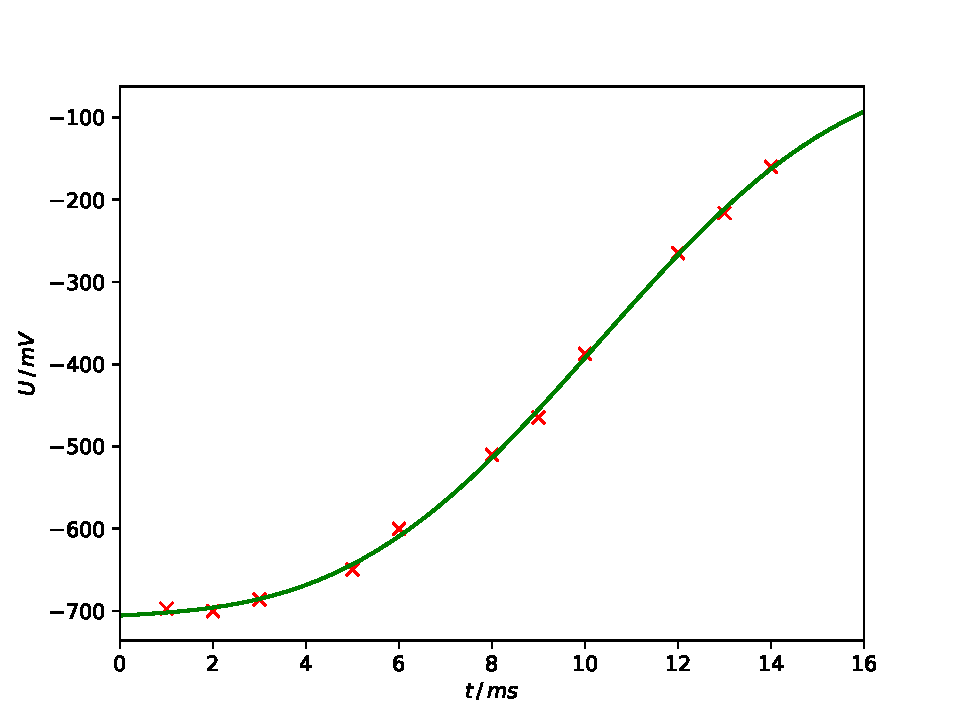
\includegraphics[width=0.9\textwidth]{Plots2/TD.pdf}
  \caption{Spannungsamplituden der Echos bei verschiedenen Pulsabständen.}
  \label{fig:D}
\end{figure}


\newpage
\subsection{Bestimmung der Viskosität und des Molekülradius}

Die Viskosität des destillierten Wassers lässt sich über
\begin{equation}
  \eta(T) = \alpha\rho(t-\delta)
\end{equation}
bestimmen, wobei $\alpha = 1.024\cdot10^{-9}\,\si{\meter\squared\per\second\squared}$
die Eichkonstante der Apparatur, $\delta = 0.5\, \si{\second}$ ein Korrekturglied
und $\rho = 997\,\si{\kilogram\per\meter\cubed}$ die Dichte des Wassers ist.
Für die gemessene Zeit von $t=898\,\si{\second}$ ergibt sich somit
\begin{equation*}
  \eta(20°C) = 0.92\,\si{\milli\pascal\second}
\end{equation*}
Mithilfe der Diffusionskonstante lässt sich nun der Molekülradius
gemäß folgender Formel bestimmen:
\begin{equation}
  r\ua{D} = \frac{k\ua{B}T}{6\pi\eta D}.
\end{equation}
Zudem kann der Molekülradius aus dem Molekülgewicht und der Dichte sowie
mithilfe des Van-der-Waal Kovolumens \cite{VdW} bestimmt werden:
\begin{align}
  r_{\text{MG}} = \left(\frac{3}{4\pi}\cdot0.74\cdot\frac{M}{\rho N\ua{A}}\right)^{1/3}\\
  r\ua{VdW} = \left(\frac{3}{4\pi}\cdot V\ua{Ko}\right)^{1/3}.
\end{align}
Für den Molekülradius erhält man mit den verschiedenen Formeln folgende
Ergebnisse:
\begin{align*}
  r\ua{D} &= (1.24\pm0.17)\,\si{\angstrom} \\
  r_{\text{MG}} &= 1.74\,\si{\angstrom} \\
  r\ua{VdW} &= 1.45\,\si{\angstrom}
\end{align*}

\newpage
\section{Diskussion}

Bei den Messungen der transversalen und der longitudinalen Relaxationszeiten lassen
sich beides Mal die aufgenommenen Datenpunkte sehr gut durch die verwendeten
Fitfunktionen beschreiben (vergleiche Abblidungen \ref{fig:T1} und \ref{fig:T2}).
Für beide Zeiten ergeben sich relativ geringe Fehler:
\begin{align*}
T\ua{1} &= (1.54\pm0.12)\,\si{s} \\
T\ua{2} &= (1.54\pm0.12)\,\si{s}.
\end{align*}
Auch bei der Bestimmung des Diffusionskoeffizienten zeigen sich nur geringe Abweichungen
von der verwendeten Fitfunktion. Zur Bestimmung des für den Koeffizienten
benötigte Halbwertsbreite wurde mehrfach bestimmt. Gegenüber des Literaturwertes
\cite{D}
für den Diffusionskoeffizienten von Sauerstoff in Wasser bei $\SI{25}{\celsius}$
ergibt sich eine geringe Abweichung von $\increment D = 9.5\,\%$:
\begin{align*}
  D &= (1.9\pm0.3)\cdot10^{-9}\,\si{\meter\squared\per\second} \\
  D\ua{lit} &= 2.1 \cdot10^{-9}\,\si{\meter\squared\per\second}.
\end{align*}
Es muss jedoch beachtet werden, dass dieses Experiment bei einer Temperatur
von $\SI{20}{\celsius}$ durchgeführt wurde. Zudem wurde schon bei Durchführung
des Experimentes deutlich, dass auch durch Ungenauigkeiten der verwendeten
Apparatur Abweichungen entstehen. Zum Beispiel schwankten die Werte für die
Halbwertbreite zwischen $\SI{95}{\milli\second}$ und $\SI{89}{\milli\second}$,
obwohl dieser Wert eigentlich konstant sein sollte.
Für die bestimmten Molekülradien zeigen sich vergleichsweise große Abweichungen
zwischen den einzelnen Methoden von bis zu $29\%$(zw. $r\ua{D}$ und $r_{\text{MG}}$):
\begin{align*}
  r\ua{D} &= (1.24\pm0.17)\,\si{\angstrom} \\
  r_{\text{MG}} &= 1.74\,\si{\angstrom} \\
  r\ua{VdW} &= 1.45\,\si{\angstrom}.
\end{align*}
Die verwendten Werte liegen jedoch alle im selben Größenbereich und passen gut zu
den Literaturwerten für die einzelnen Molekülradien von Wasserstoff und Sauerstoff.
